\chapter{Análise Bibliográfica sobre Programação Competitiva, por Enzo Yoshio}

\section{Planejamento do estudo}

    O planejamento de estudos é importante para os estudos científicos e o método científico pois sem um planejamento e questionamento do que a pesquisa deve procurar, o objetivo e o foco da pesquisa pode se perder sem esse planejamento e a organização dos pesquisadores feita previamente. Dito isso, durante o planejamento, é necessário levantar alguns questionamentos para nortear a pesquisa e ficar claro pros pesquisadores o alvo de pesquisa e o que eles devem solucionar. Em sequência há alguns questionamentos feitos para essa análise bibliográfica.
 

\begin{itemize}
    \item Qual a relevância da programação competitiva para a comunidade científica? 
    \item A programação competitiva tem influenciado a comunidade científica e o mercado de trabalho?
    \item A programação competitiva vem sendo popularizada nos últimos anos?
\end{itemize}

\subsection{Limitações} O artigo foi proposto em uma matéria semestral na Universidade de Brasília, sendo feito como atividade semanal para aprender os usos do R Studio e bibliometrix. Logo houve pouco tempo para o desenvolvimento do artigo buscando as fontes necessárias para que ficasse um artigo substancial e bem feito. O artigo foi feito ao longo de uma semana, usando um horário de 10 horas aproximadamente.

\section{Coleta de dados}

A coleta de dados foi realizada usando o software de busca Web Of Science no dia 8 de fevereiro de 2022, acessado por meio do Portal de Periódicos da Capes.

\subsection{Query de Busca}

Para a busca, foi usada uma \query\ abaixo:
\begin{verbatim}
(codeforces)
(compet* and program*)
(codechef)
\end{verbatim}

\subsubsection{Explicação para os termos de busca usados}

Como o foco era programação competitiva, o termo compet* e program* foram usados concatenados para buscar todas as referencias possíveis a programação competitiva, também foram usados os nomes de alguns sites famosos que a comunidade de programação científica usa bastante, sendo o mais famoso o codeforces. Não há um consenso em qual nome oficial deveria ser usado para programação competitiva, por exemplo, no Brasil também é conhecida como Maratona de Programação, algumas pessoas influentes nessa comunidade já usaram outros termos como sport of mind, programming sports, entre outros, mas definitivamente o mais famoso é competitive programming e esse é o motivo ao qual foi usado na query apenas o mais famoso, visto que os outros termos são muito pouco utilizados e não são famosos, logo a busca por esses termos não traria bons resultados na query, podendo até mesmo atrapalhar e trazer resultados indesejados, por isso a escolha de fazer a query apenas com o nome mais conhecido desse hobby e também de seus principais sites, visando a citação deles correlacionado com a programação competitiva.

\subsection{Registros recuperados}

Os 5000 registros obtidos na busca podem ser encontrados no link \url{}
Foi utilizada o opção de exportação para aquivo de texto sem formatação, contemplando todos as 29 opções de campo. Os 5000 registros foram recuperado em grupos de 1000 para posteriormente serem concatenados em um único arquivo para que o bibliometrix pudesse processá-lo.

Foram utilizadas as opções \textit{Exportar registros para arquivo de texto sem formatação} e \textit{export full record / Gravar Conteúdo: Seleção personalizada, com todos os 29 campos disponíveis, inclusive referências citadas} no Word Of Science, para que as citações também fossem usadas em análises da citações (estrutura intelectual do conhecimento). Os 5000 registros foram recuperados em 5 blocos de até 1.000 registros por vez (1-1000, 1001-2000, 2001-3000, 3001-4000, 4001-5000).

\section{Análise dos dados}

\subsection{Filtragem de registros}
Para uma melhor análise, é possível fazer o uso de filtros sobre os dados bibliométricos.

Aplicou-se uma filtragem ao \dataset prévio, com 5000 registros, em que havia prévias de artigos, artigos de conferência, capítulos de livro, entre outros... Manteve-se apenas no \dataset os artigos que foram publicados em revistas de cunho científico.\footnote{Supõe-se que os conhecimentos de maior qualidade sobre o tema em questão está nas publicações feitas em revistas.}.  Logo após aplicar essa filtragem pelo bibliometrix, 3164 registros continuaram no \dataset, que seguirá fazendo alguns processos e filtragens no bibliometrix.

Todos os documentos recolhidos tiveram uma filtragem para restar apenas os artigos que podem se encaixar como artigos os quais foram publicados em revistas científicas. Após essa filtragem, também foram tratados sob a lei de Bradford. Dos 3164 arquivos já filtrados, foram filtrados novamente para 1361 que são os documentos que serão relevantes para a análise bibliográfica sobre programação competitiva.

\subsection{Análise descritiva do \dataset\   }

Constam as informações gerais sobre os conjuntos de dados:
As informações mais gerais sobre o \dataset\   são as seguintes:
\begin{description}
    \item [\textit{Timespan}] Os artigos obtidos da busca após a filtragem foram publicados entre o período de 1991 até 2022
    \item [\textit{Sources (Journals, Books, etc)}] Os artigos possuem ao todo 163 fontes diferentes, sendo assim, em média, 8 artigos por revista.
    \item [\textit{Average years from publication}] A média de tempo de publicação dos artigos é de 5.5 anos
    \item [\textit{Average citations per documents}] A média de citações por documentos é 10.43.
    \item [\textit{Average citations per year per doc}] Após o ano de sua publicação, das um dos dos artigos foi citado em média 1.283 vezes por ano.
    \item [\textit{References}] Ao todo, foram feitas 46173  referências por entre os artigos coletados
    \item [\textit{Keywords Plus (ID)}] 2153 palavras chaves do tipo ID (Keyword Plus)
    \item [\textit{Author's Keywords (DE)}]  4383 palavras chaves escolhidas pelos autores dos artigos

    \item [\textit{Authors}]  
    \item [\textit{Author Appearances}] 
    \item [\textit{Authors of single-authored documents}] Dos 5223 autoes, 95 escreveram artigos individualmente
    \item [\textit{Authors of multi-authored documents}] Dos 5223 autores, 5138 são autores de artigos escritos em colaboração com outros.
    \item [\textit{Single-authored documents}] Dos 1361 documentos, 95 foram escritos indidualmente, o que sobrou foram produzidos em co-autoria.
    \item [\textit{Documents per Author}] A média de documentos por autor é de 0.26
    \item [\textit{Authors per Document}] A média de autores por documento é de 3.84.
    \item [\textit{Co-Authors per Documents}] As 5749 aparições de autores se distribuem em 4.22 por documento
    \item [\textit{Collaboration Index}] O indíce de colaboração (total de autores em artigos escritos em co-autoria / total de artigos escritos em co-autoria) é de 4.06.
\end{description}

As informações podem ser encontradas também na imagem abaixo:

\begin{figure}[ht]
    \centering
    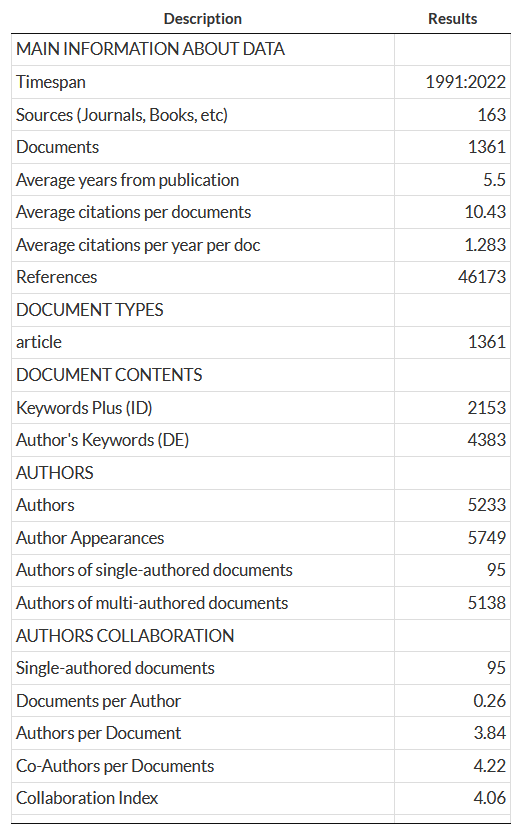
\includegraphics[width=12cm]{experiments/enzoyoshio/AnaliseBibliometrica/mainInformation.PNG}
    \caption{ Principais informações sobre os dados coletados }
    \label{fig:mainInfo}
\end{figure}


\subsection{Evolução da Produção Científica}

\begin{figure}[ht]
    \centering
    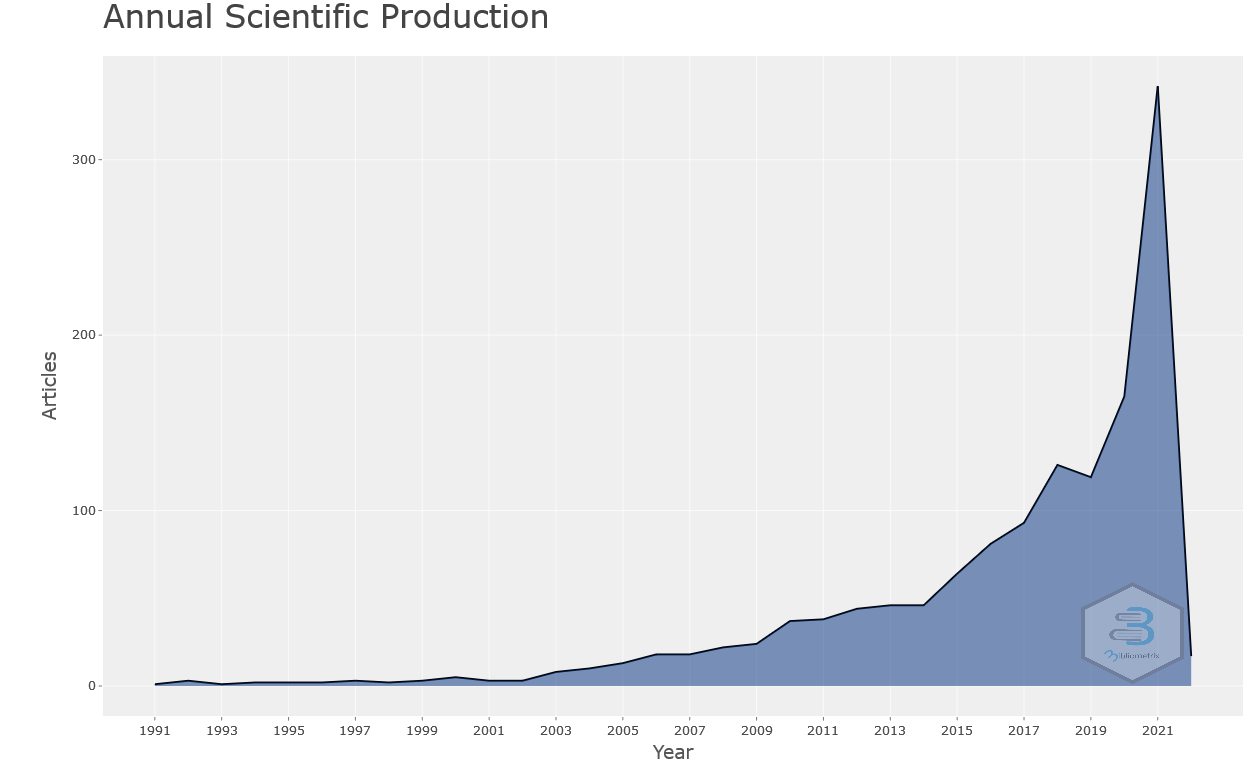
\includegraphics[width=12cm]{experiments/enzoyoshio/AnaliseBibliometrica/anualScientificProduction.png}
    \caption{ Produção científica anual do \dataset\ }
    \label{fig:evoEnzoYoshio}
\end{figure}

Como pode ser observado no gráfico:

Até o ano de 2000 as publicações eram praticamente inexistentes, visto que a popularização da programação competitiva foi apenas nos anos 2000, principalmente pelo fato da criação e popularização da internet. Quanto mais pessoas começaram a ter acesso a internet, mais pessoas puderam conhecer essa nova área conhecida como computação. Logo, após os anos 2000 pudemos observar uma curva que cresce a cada ano, tendo no ano de 2021 tido seu pico de publicações e provavelmente essa curva só tende a crescer, pois mais e mais pessoas estão ingressando no mundo da programação competitiva, seja ela por ajudar em entrevistas de emprego, ou apenas pelo simples fato de conseguir aprender coisas novas e treinar o raciocínio lógico. 

\subsection{Evolução das Citações}

\begin{figure}[ht]
    \centering
    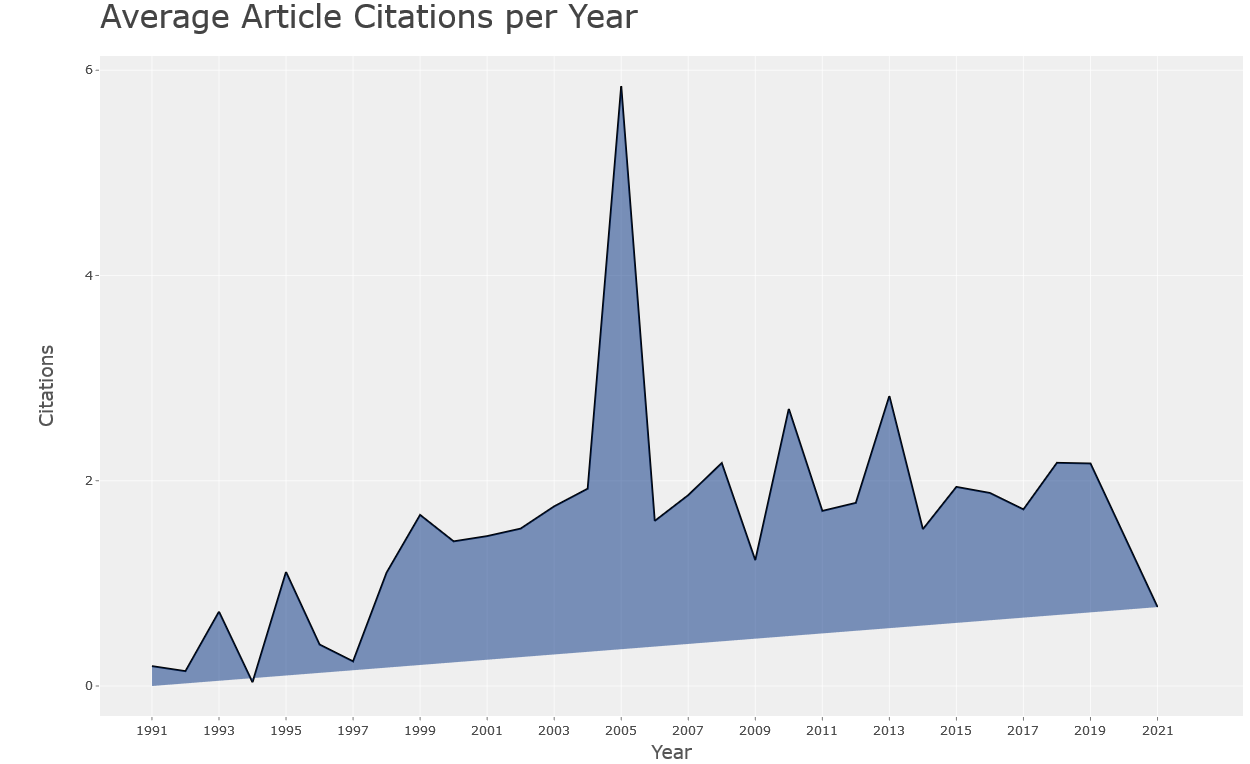
\includegraphics[width=12cm]{experiments/enzoyoshio/AnaliseBibliometrica/averageCitationPerYear.png}
    \caption{ Média de citação anual do \dataset\ }
    \label{fig:citaEnzoYoshio}
\end{figure}

A figura em \ref{fig:citaEnzoYoshio} revela quantas citações foram feitas, em média, ao longo do ano. A curva é levemente crescente e percebe-se um leve aumento a cada ano, percebe-se que há um pico em 2006, pois provavelmente foi publicado um artigo bem conceituado na área e importante para o desenvolver da área nos anos seguintes. Percebe-se uma leve queda no ano de 2021, mas isso é de se esperar, pois ainda não foram feitas referências sobre esse ano ainda. Com isso, é interessante observar essa curva de citações por ano, para entender melhor como se desenvolve essa área.

\subsection{\textit{Gráfico de três campos}}

O gráfico em \ref{fig:} mostra um gráfico de três campos feitos com os dados acerca das referências, autores e palavras-chaves mais relevantes.

\begin{figure}[ht]
    \centering
    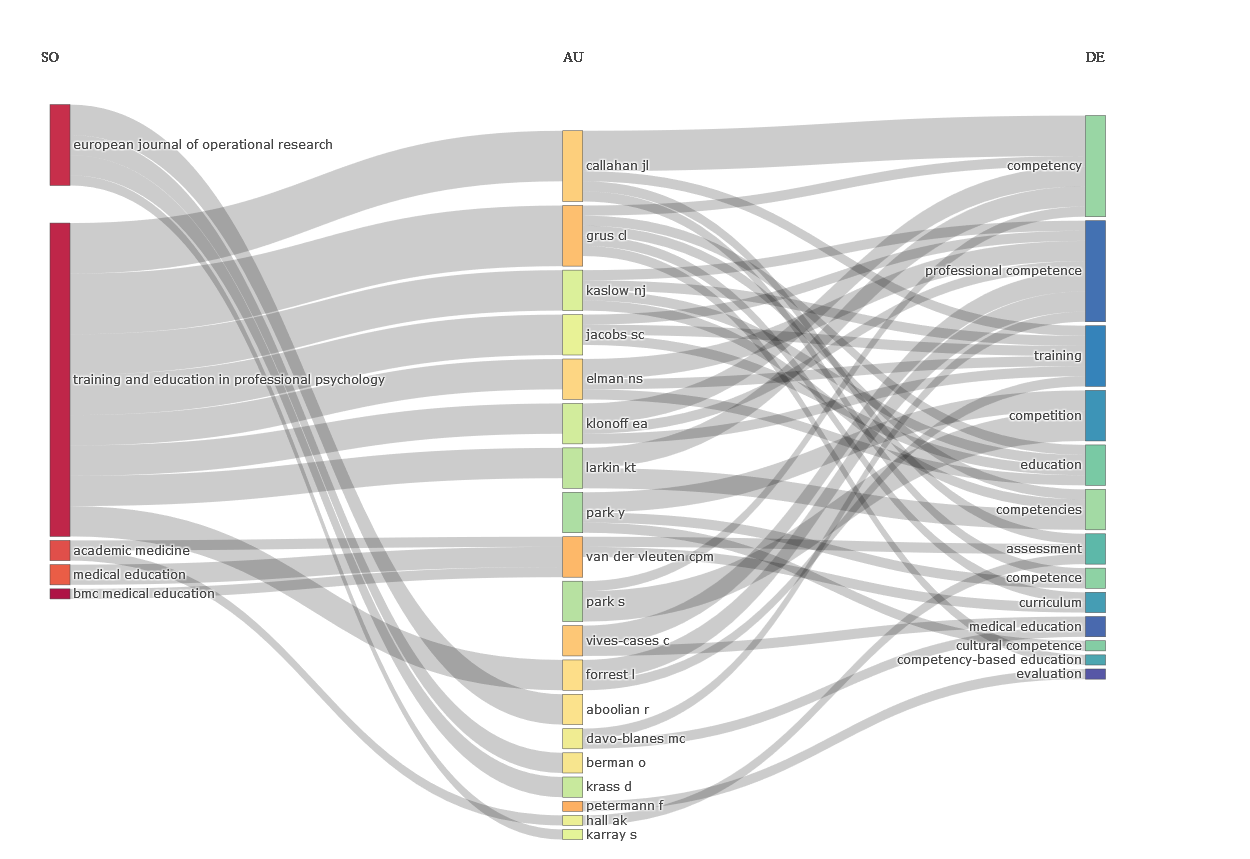
\includegraphics[width=12cm]{experiments/enzoyoshio/AnaliseBibliometrica/threeFieldsPlot.png}
    \caption{Gráfico de três campos analisando palavras-chave no \textit{db\_GPU}}
    \label{fig:threeFieldEnzoY}
\end{figure}

Observando as palavras mais relevantes, podemos ver que tem muitos artigos em que as palavras-chave também incluem a educação, logo é importante notar a correlação entre programação competitiva e o aprendizado de alunos na graduação.

Vale ressaltar também que, há algumas palavras chaves diferentes, tendo em vista que o tema pode abordar diferentes assuntos, é complicado de fazer um filtro justamente pelo conteúdo poder abordar muitas coisas, porém podemos ver uma agregação entre os autores mais citados e as palavras-chave e suas referências.